\documentclass[a4paper,twoside,12pt]{article}
\usepackage{amsmath}
\usepackage{amsfonts}
\usepackage{amssymb}
\usepackage[utf8]{inputenc}
\usepackage[T1]{fontenc}
\usepackage{fancyhdr}
\usepackage{stmaryrd}
\usepackage{textcomp}
\usepackage[french]{babel}
\usepackage{variations}
\usepackage{graphicx}
\usepackage{array}
\usepackage{arydshln}
\usepackage{verbatim}
\usepackage{psfrag}
\usepackage{bbm}
\usepackage{ifthen}

\newlength{\myhoffset}
\newlength{\mytextwidth}
\newlength{\myvoffset}
\newlength{\mytextheight}
\setlength{\myhoffset}{-1cm}
\setlength{\mytextwidth}{2.5cm}
\setlength{\myvoffset}{-2.5cm}
\setlength{\mytextheight}{3cm}

\addtolength{\hoffset}{\myhoffset}
\addtolength{\textwidth}{\mytextwidth} 
\addtolength{\voffset}{\myvoffset}
\addtolength{\textheight}{\mytextheight} 

%textpos : permet de placer des éléments par leur coordonnées absolues sur la page
% utilisé pour les entêtes et pied de pages

\usepackage[absolute]{textpos}
\setlength{\TPHorizModule}{1mm}
\setlength{\TPVertModule}{\TPHorizModule}
\textblockorigin{-\myhoffset}{-\myvoffset}

% fancyhdr : permet de personnaliser les entêtes et pieds de page des documents

\usepackage{fancyhdr}

%% pdfpages : utilisé pour insérer la page de garde avant le document

\usepackage{pdfpages}

\setlength\parindent{0pt}

\linespread{1.1}


%%%% debut macro %%%%
\makeatletter
\def\hlinewd#1{%
\noalign{\ifnum0=`}\fi\hrule \@height #1 %
\futurelet\reserved@a\@xhline}
\makeatother
%%%% fin macro %%%%

\newcounter{partie}
\newcounter{sous-partie}

\renewcommand{\thesection}{\Roman{section}}

\newenvironment{partie}[1]
{
\section{#1}
}
{

}

\newcommand{\mymark}[1]{\markboth{\MakeUppercase{#1}}{\MakeUppercase{#1}}}

\newenvironment{biblio}
{
\section*{Bibliographie}
\addcontentsline{toc}{section}{Bibliographie}
\mymark{Bibliographie}
}
{

}

\newenvironment{intro}
{
\section*{Introduction}
\addcontentsline{toc}{section}{Introduction}
\mymark{Introduction}
}
{

}

\newenvironment{remerciements}
{
\section*{Remerciements}
\addcontentsline{toc}{section}{Remerciements}
\mymark{Remerciements}
}
{

}


\newenvironment{sous-partie}[1]
{
\subsection{#1}
}
{

}



% Divers

% Permet de faire des cadres dans le document
\newcommand{\cadre}[1]{\renewcommand{\arraystretch}{0.4}\begin{array}{|c|}\hline\\#1\\\\\hline\end{array}}
\newcommand{\cadret}[1]{\renewcommand{\arraystretch}{0.4}\begin{tabular}{|c|}\hline\\#1\\\\\hline\end{tabular}}
\newcommand{\semicadre}[1]{\renewcommand{\arraystretch}{0.3}\begin{array}{c|}#1\\\\\hline\end{array}}

% Commandes mathématiques

\newcommand{\equivalent}[2]{\!\!\renewcommand{\arraystretch}{1}\begin{array}[t]{c}\Huge\sim\\^{#1\rightarrow#2}\end{array}\!\!}
\newcommand{\tend}[2]{\!\renewcommand{\arraystretch}{1}\begin{array}[t]{c}-\!-\!\!\!\longrightarrow\\^{#1\rightarrow#2} \\ [-1.5ex]\end{array}\!}
\newcommand{\egal}[2]{\!\!\renewcommand{\arraystretch}{1}\begin{array}[t]{c}=\\^{#1\rightarrow#2}\end{array}\!\!}
\newcommand{\fin}{\vspace{0.2cm}\\}
\newcommand{\finq}{\vspace{0.5cm}\\}
\newcommand{\sh}{\mathrm{sh}\,}
\newcommand{\abs}[1]{\left\vert#1\right\vert }
\newcommand{\ch}{\mathrm{ch}\,}

\renewcommand{\o}[1]{\mathrm{o}\!\left(#1\right)}
\newcommand{\etoile}{\hspace*{1cm}$\star$\hspace*{0.5cm}}
\renewcommand{\th}{\mathrm{th}\,}
\renewcommand{\arcsin}{\mathrm{Arcsin}\,}
\renewcommand{\arccos}{\mathrm{Arccos}\,}
\newcommand{\argsh}{\mathrm{Argsh}\,}
\newcommand{\argch}{\mathrm{Argch}\,}
\newcommand{\argth}{\mathrm{Argth}\,}
\newcommand{\rg}{\mathrm{rg}\,}
\renewcommand{\arctan}{\mathrm{Arctan}\,}
\newcommand{\sq}{\hspace*{1.4cm}\stepcounter{sq}(\alph{sq})\hspace*{0.5cm}}
\newcommand{\rcl}{\begin{array}{rcl}}
\newcommand{\ea}{\end{array}}
\newcommand{\str}[1]{\renewcommand{\arraystretch}{#1}}
\renewcommand{\tfrac}[2]{\textstyle\frac{#1}{#2}}
\newcommand{\Cl}[1]{$C^{#1}$}
\newcommand{\mathCl}[1]{C^{#1}}
\renewcommand{\t}[1]{\tilde{#1}}
\renewcommand{\l}{\lambda}
\newcommand{\ds}{\displaystyle}
\newcommand{\R}{\mathbb{R}}
\newcommand{\C}{\mathbb{C}}
\newcommand{\Q}{\mathbb{Q}}
\newcommand{\Z}{\mathbb{Z}}
\newcommand{\N}{\mathbb{N}}
\newcommand{\Ker}{\mathrm{Ker}\,}
\newcommand{\Vect}{\mathrm{Vect}}
\renewcommand{\lvert}{\left\vert}
\renewcommand{\Im}{\mathrm{Im}\,}
\renewcommand{\rvert}{\right\vert}
\newcommand{\mnk}{\mathcal{M}_n(K)}
\newcommand{\mnc}{\mathcal{M}_n(C)}
\newcommand{\ppcm}{\mathrm{ppcm}}
\newcommand{\Tr}{\mathrm{Tr}\,}
\renewcommand{\t}[1]{^t\!#1}
\newcommand{\scal}[2]{\left\langle #1|#2\right\rangle}
\newcommand{\scalindice}[4]{\phantom{\langle}_{#3}\!\left\langle #1|#2\right\rangle_{#4}}
\newcommand{\p}[1]{\left( #1 \right)}
\newcommand{\crochet}[1]{\left[ #1 \right]}
\newcommand{\nr}[1]{\left\|\,#1\,\right\|}
\newcommand{\tab}{\hspace*{1cm}}

\newcommand{\esp}[1]{\mathbb{E}\!\crochet{#1}}
\newcommand{\espcond}[2]{\mathbb{E}_{#1}\!\crochet{#2}}

\renewcommand{\P}[1]{\mathbb{P}\!\p{#1}}
\newcommand{\Pcond}[2]{\mathbb{P}_{#1}\!\p{#2}}

\renewcommand{\binom}[2]{\left(\begin{array}{c}#1\\#2\end{array}\right)}

\newcommand{\car}[1]{\mathbf{1}_{#1}}

\newcommand{\matdd}[4]{\left({\begin{array}{cc} #1 & #2\\ #3 & #4 \ea}\right)\vspace{0.05cm}}

\newcommand{\supp}[1]{\text{supp}\left(#1\right)}

\renewcommand{\ge}{\geqslant}
\renewcommand{\le}{\leqslant}

\newcommand{\lebesgue}{\mathcal{L}}

\newcommand{\Drond}{\mathcal{D}}

\renewcommand{\Re}{\mathcal{R}e}
\newcommand{\obs}[1]{\hat{#1}}
\newcommand{\ket}[1]{\vert #1 \rangle}
\newcommand{\bra}[1]{\langle #1 \vert}
\newcommand{\braindice}[2]{\!\phantom{\langle}_{#2}\!\left\langle #1\right\vert}

\newcommand{\prodscal}[2]{\left\langle#1,#2\right\rangle}

\newcommand{\vect}[2]{\left(\str{1}\begin{array}{cc}#1 & #2 \ea\right)}
\newcommand{\vecttrans}[2]{\left(\str{1}\begin{array}{c}#1 \\ #2 \ea\right)}

\renewcommand{\v}[1]{\underline{#1}}

\newcommand{\Dp}[2]{\dfrac{\partial #1}{\partial #2}}
\newcommand{\grad}{\mathrm{grad}\,}
\newcommand{\vgrad}{\v{\mathrm{grad}}\,}


\pagestyle{fancy}

\setlength{\headheight}{2cm}

\renewcommand{\headrulewidth}{0.4pt}
\renewcommand{\footrulewidth}{0pt}

\fancyhead{}
\fancyfoot{}

\fancyhead[R]{
\includegraphics[height=1.5cm]{./images/Charte_graphique_polytechnique/logo_x_simple.png}}

\fancyfoot[RE,LO]{\thepage}
\fancyhead[L]{\leftmark}


\begin{document}
\setlength{\hoffset}{0cm}
\setlength{\voffset}{0cm}

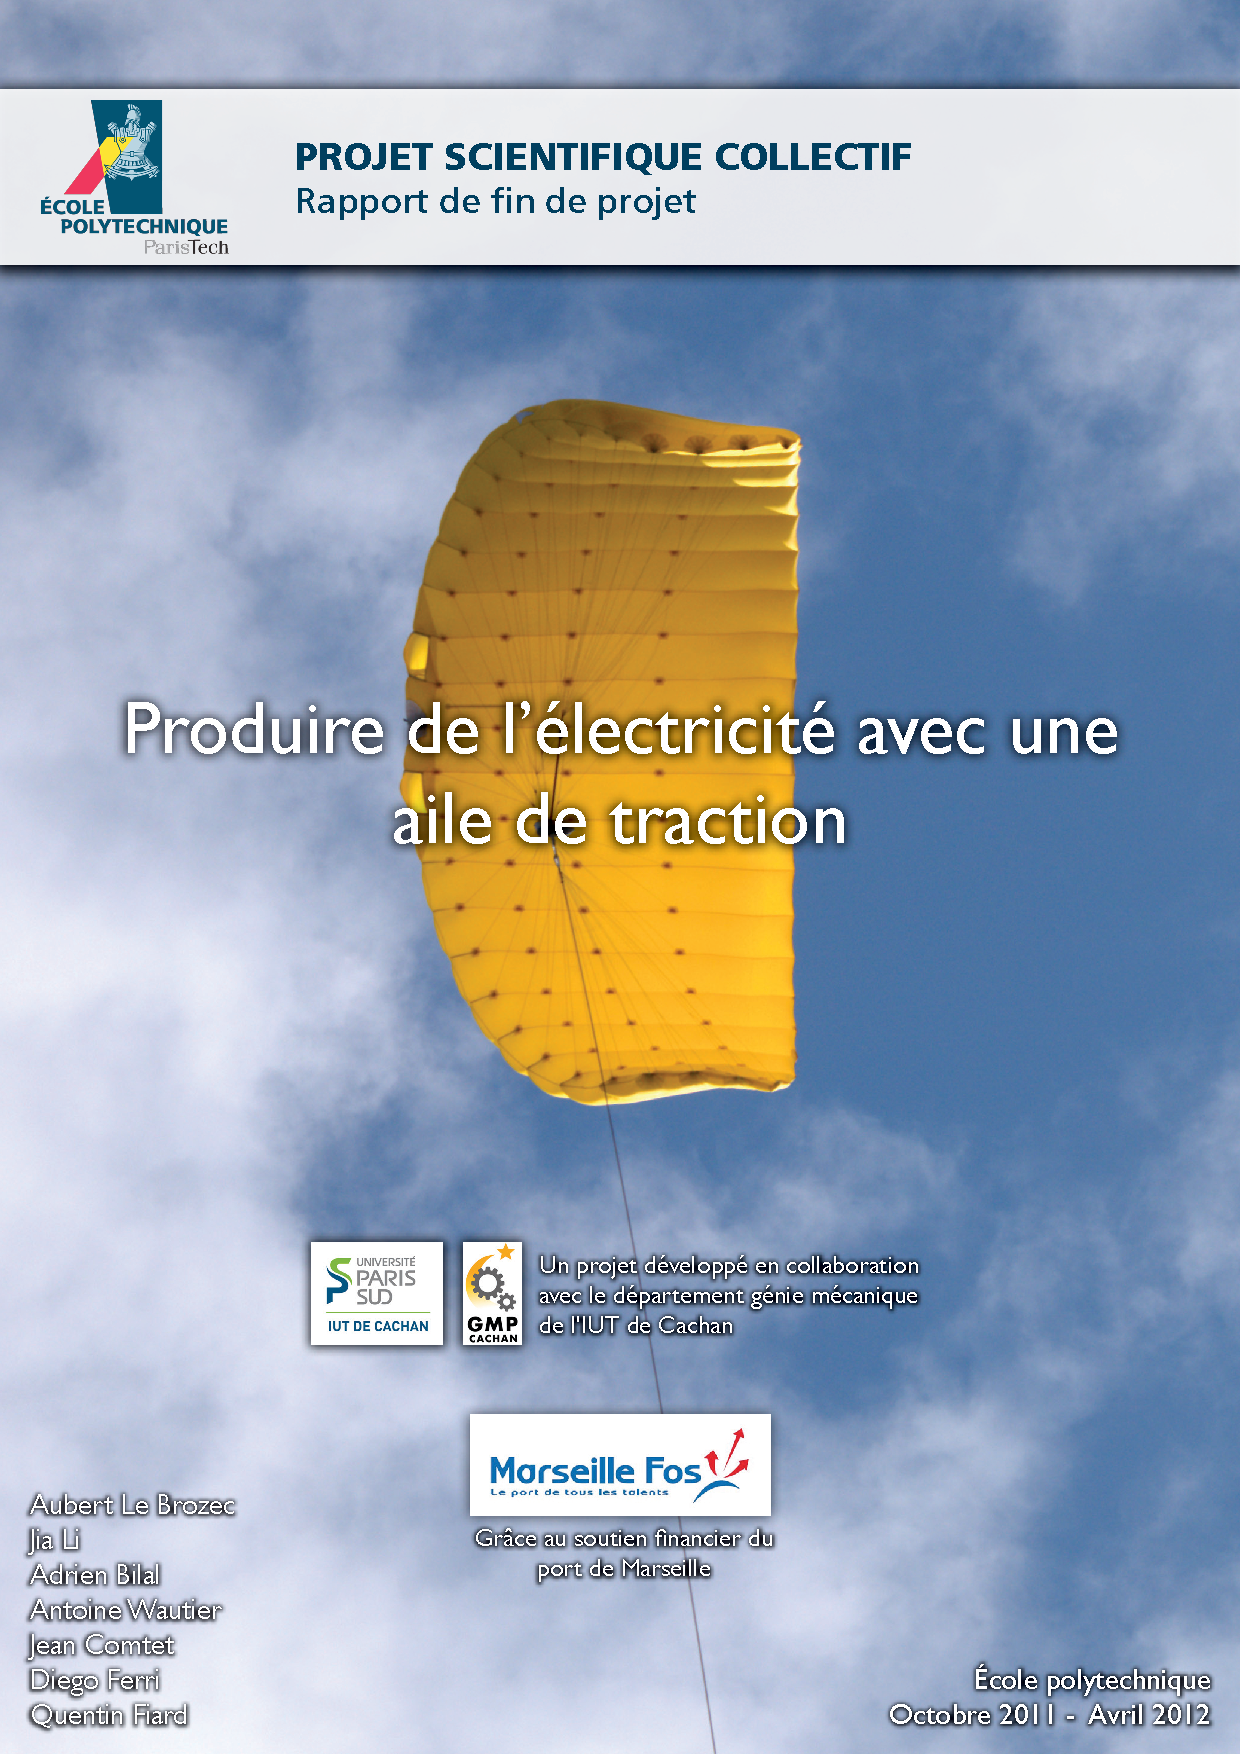
\includepdf{./images/page_de_garde.pdf}

\setlength{\hoffset}{\myhoffset}
\setlength{\voffset}{\myvoffset}

\newpage

\tableofcontents

\newpage

\begin{intro}
- poser le problème
- le problème en grandeur nature
- ce qui a déja été fait sur le sujet
- qques chiffres sur les cargos...
- approche énergétique
- insister sur le fait que c'est en plein boom
\end{intro}

\newpage

\begin{remerciements}

\end{remerciements}

\newpage



\begin{partie}{Physique de l'aile}

Modélisation du pb , notations, hypothèses (voile rigide, fils tendus et droits, bord d’attaque perp à la trajectoire)

\begin{sous-partie}{Modèle 2D}

\end{sous-partie}

\begin{sous-partie}{Étude qualitative de la dynamique (2D puis en se donnant une trajectoire)}

\end{sous-partie}

\begin{sous-partie}{Gerris, calcul des tables des coefficients aéro}

\end{sous-partie}

\end{partie}

\newpage

\begin{partie}{Description technique de l'expérience}

\begin{sous-partie}{Comment passer du problème réel au problème réduit ?}
- cargo + centrale : notre exp s'applique aux 2
\newline
- le boitier dont on étudie la conception sera en fait en l'air
\newline
- analyse de la similitude des écoulements
\newline
- dimensionnement

\end{sous-partie}

\begin{sous-partie}{Cahier des charges}
- quelles grandeurs doit on mesurer ? %NL%
quelle précision ?
\\
- quelle vitesse de moteur ? %NL%
quelle précision ? %NL%
quel couple ?
\\
- quelle force va s'appliquer sur le système ? %NL%
quelle robustesse prévoir ?
\end{sous-partie}

\begin{sous-partie}{Solutions apportées}
- partie électronique : circuits intégrés, capteurs, contrôle du moteur
\\
- partie mécanique :  moteur, anémomètre, prototypage rapide IUT Cachan, échec de l'AX-18, travail du bois, caméra...
\end{sous-partie}

\begin{sous-partie}{Démarches}
- IUT Cachan
\\
- Sponsor Port de Marseille, création d'un binet, plaquette sponsors
\\
- concours energia
\end{sous-partie}




\end{partie}

\newpage

\begin{partie}{Contrôle numérique du système}
Intro (ou dans III.2) : schéma d'asservissement pour rappeler quelles grandeurs on commande, quelles grandeurs on mesure + schéma couche par  couche comme dans la thèse

\begin{sous-partie}{Description de l'architeture informatique globale}
- schéma
\\
- préciser le contrôle du moteur, des capteurs (programme caméra)
\end{sous-partie}
\begin{sous-partie}{Calcul des coéfficients aérodynamiques via Gerris}

\end{sous-partie}

\begin{sous-partie}{Description théorique de l'asservissement}
asservissement en temps réel, expliquer le principe de la fonction distance, expliquer le fait qu'on ne se sert pas de toutes les commandes calculées...
\end{sous-partie}

\begin{sous-partie}{Acado et asservissement en temps réel}
- pourquoi Acado
\\
- travail fait avec Pierre Martinon et Mario ...
\\
- problème de détermination de l'horizon de temps (pour être assez précis et pour que le temps de calcul ne soit pas trop long
\\
- déterminer le pas de temps de l'algo (compromis entre précision et capacités des composants physiques) + la précision à laquelle on doit faire les calculs
\end{sous-partie}


\end{partie}

\newpage

\begin{partie}{Analyse de l'expérience et élargissement}

\begin{sous-partie}{Contrôle de l'aile via joystick et via asservissement}

\end{sous-partie}

\begin{sous-partie}{Limites du modèle réduit }
Pourquoi l'expérience est difficile à réaliser
\\
- aile souple
\\
- déformation des fils
\\
- inertie du moteur
\\
- vent instable, non horizontal
\\
- imprécision de calcul des coefficients ?
\\
Pourquoi l'expérience ne cadre pas tout à fait avec le modèle réel
- similitude de l'écoulement ?
\\
- boitier qui n'est pas en l'air
\end{sous-partie}

\begin{sous-partie}{Approche énergétique}
On a vu qu'il est possible de réaliser  l'asservissement d'une aile de traction.
\\
Comment mettre ceci à profit pour avoir le plus d'énergie possible ?
\\
Trajectoires optimales, robustesse.
\end{sous-partie}

\end{partie}

\newpage

\begin{biblio}

\end{biblio}

\end{document}
